\documentclass[spanish,10pt,a4paper,final,onecolumn,leqno,fleqn]{article}
\usepackage[utf8]{inputenc}
\usepackage[T1]{fontenc}
\usepackage[left=2.00cm, right=2.00cm, top=2.00cm, bottom=2.00cm]{geometry}
\usepackage{babel}
\usepackage{graphicx}
\graphicspath{{Fotos/},{Dibujos/},{Apoyo/}}
\title{Análisis y resultados}
\author{Uriel Grimaldi Diaz }
\begin{document}

\maketitle
\section{Experimento IV.}

Primeramente, antes de comenzar a realizar las observaciones del experimento, conozcamos la maquina que utilizamos para cargar nuestros electrodos, el generador de Van Graaff.

El funcionamiento es sencillo, un motor hace rodar una cinta sobre los rodillos que están hechos de material aislante que debido a la fricción acaban cargados, en el caso de la cinta, queda cargada negativamente por el interior y en el exterior de forma positiva.

En la parte superior e inferior existe un peine que reúne las cargas positivas, esto lo hace porque el rodillo superior queda cargado de forma positiva y repele a las cargas positivas en la cinta hacía el peine.Cuando la cinta regresa mantiene la carga negativa en su interior y esta carga es acumulada por el otro peine. Con esto podemos concluir que la polaridad es positiva en la superficie de la esfera metálica y negativa en la base del generador.

\begin{figure}[h!]
	\centering
	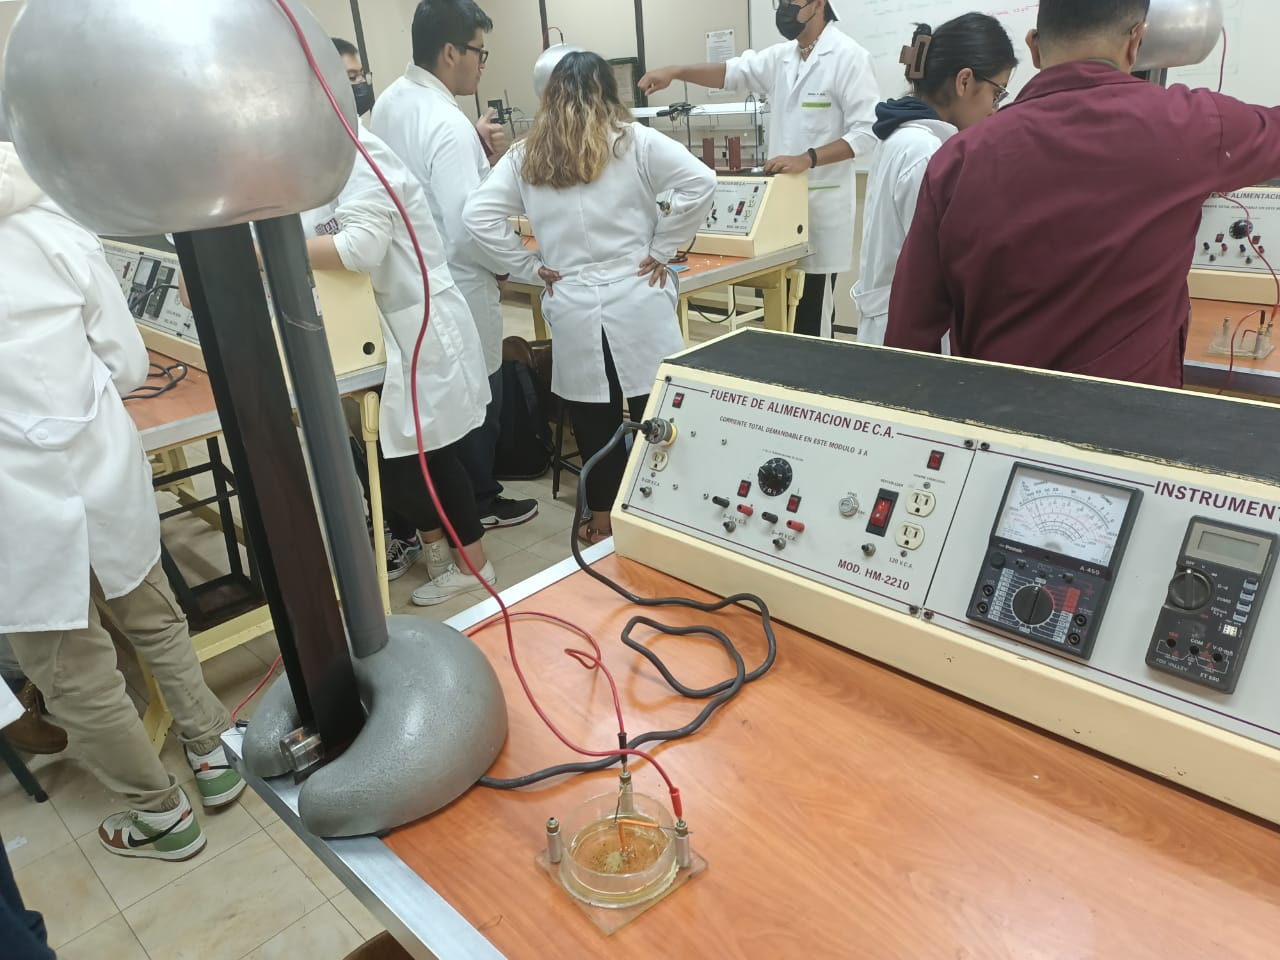
\includegraphics[scale=0.2]{Generador 2}
	\caption{Generador de Van Graaff}
	\label{fig:Generador}
	Observe que la punta roja es positiva y la punta negra negativa.
\end{figure}

Con esto aclarado, podemos comenzar a analizar los campos formados por la interacción de los pares de electrodos.

\newpage
\subsection{Lenteja y arillo.}



La lenteja y el arillo poseen carga contraria.

\begin{figure}[h!]
	\centering
	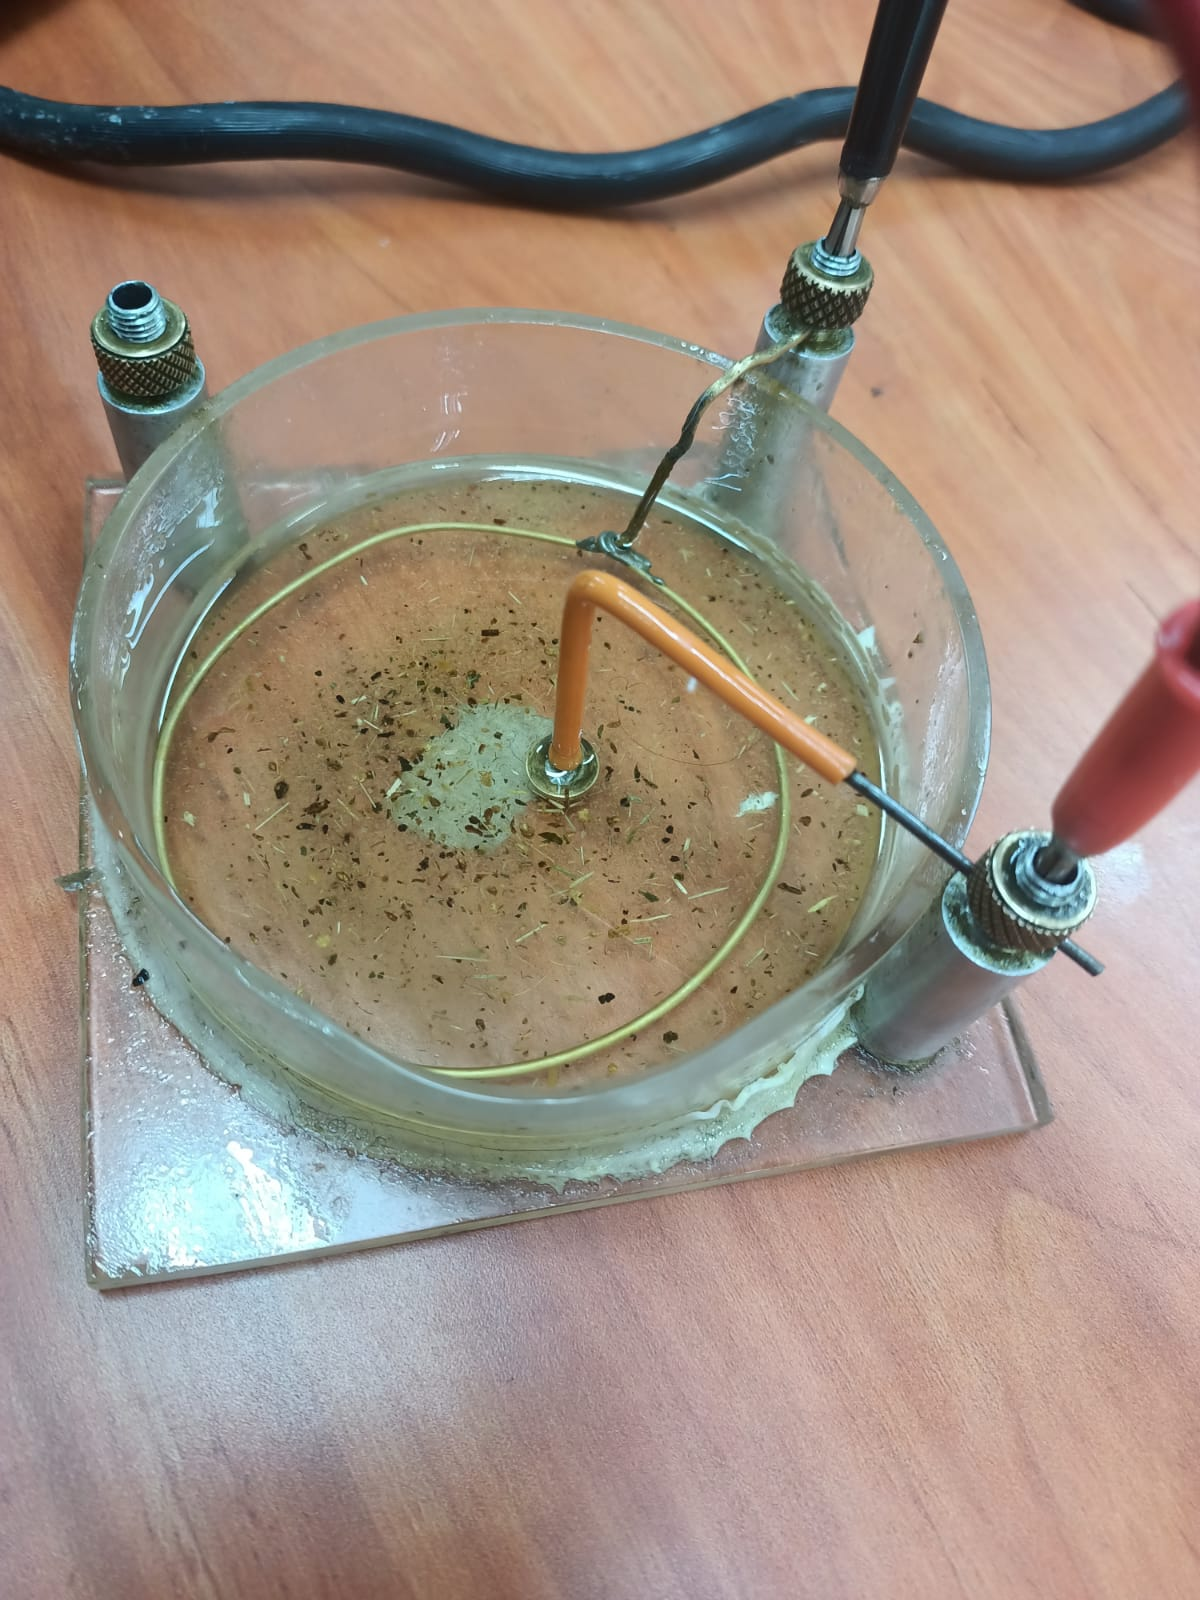
\includegraphics[scale=0.15]{Lenteja y anillo 1}
	\caption{Sistema con el generador apagado.}
	\label{fig:AyLO}
\end{figure}


\begin{figure}[h!]
	\centering
	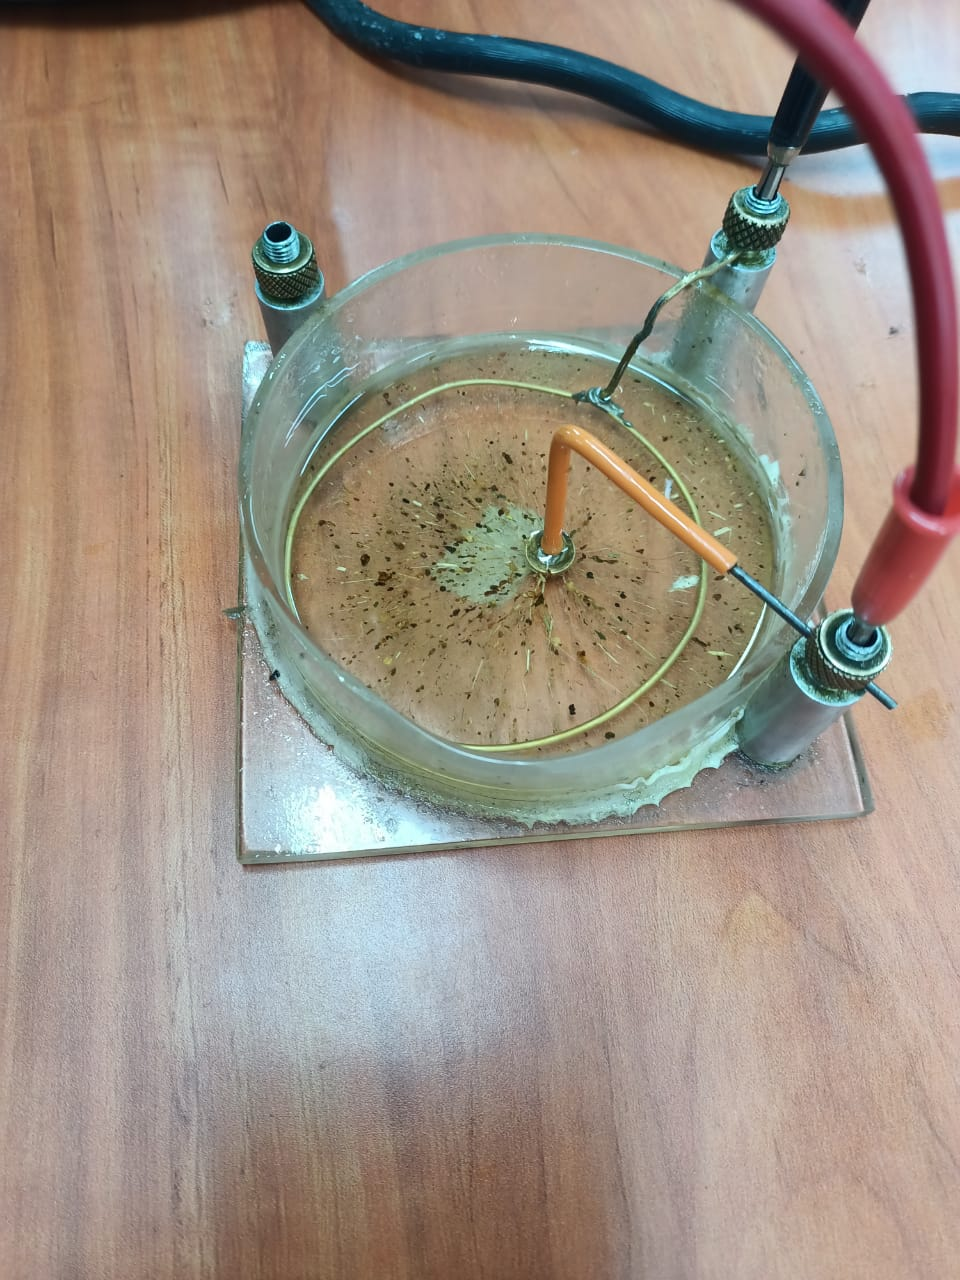
\includegraphics[scale=0.2]{Lenteja y anillo 2.1}
	\caption{Sistema con el generador encendido.}
	\label{fig:AyLE1}
\end{figure}

En la figura \ref{fig:AyLE1} se puede apreciar como el aserrín comienza a formar líneas al rededor de la lenteja y por fuera del anillo. Podemos notar también que según lo observado en la figura \ref{fig:Generador} el anillo posee una carga negativa y la lenteja positiva.

\newpage
\begin{figure}[h!]
	\centering
	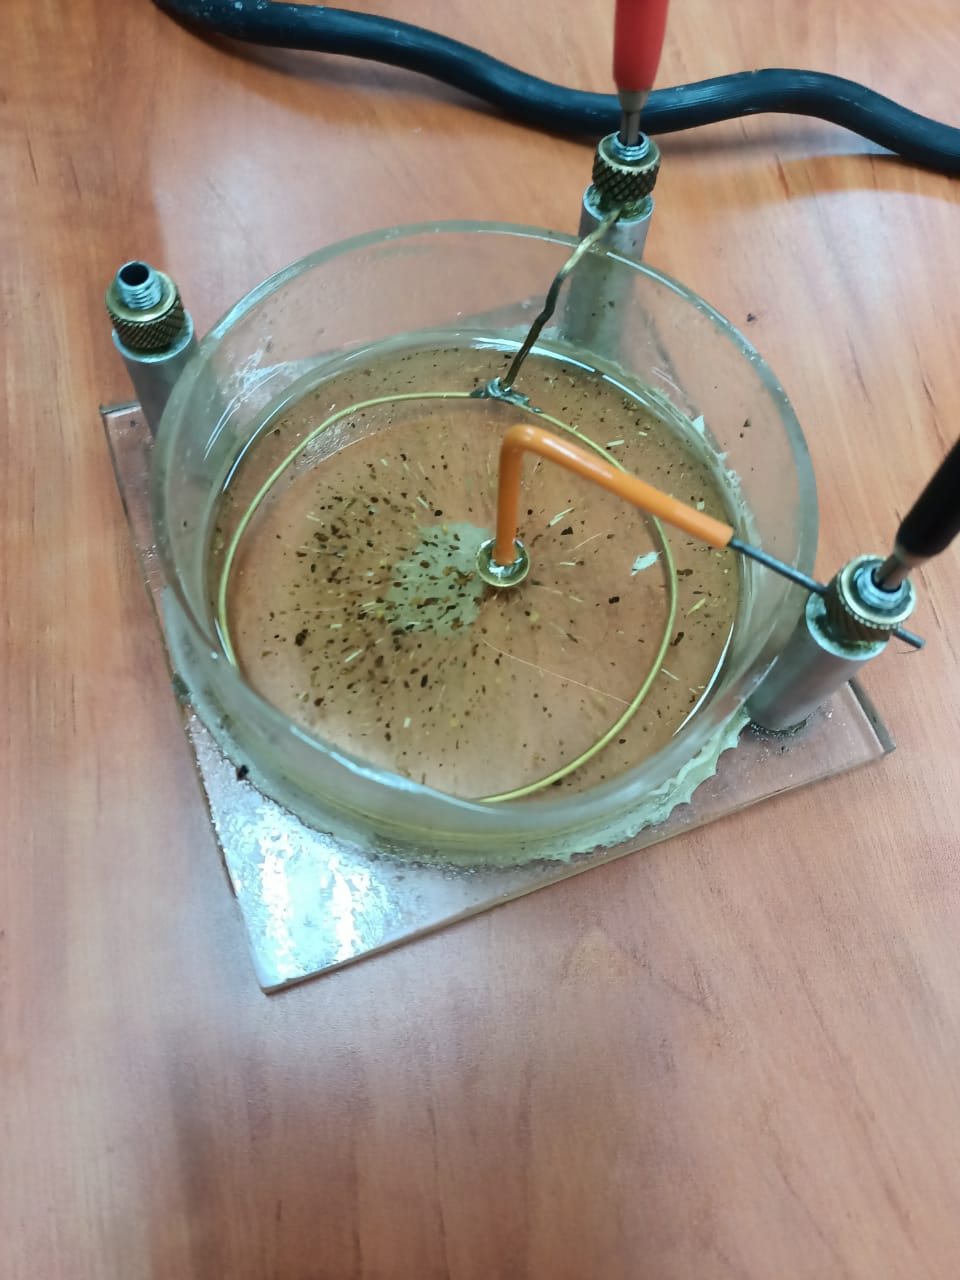
\includegraphics[scale=0.2]{Lenteja y anillo 2}
	\caption{Sistema con la polaridad invertida y el generador encendido.}
	\label{fig:AyLE2}
\end{figure}

En la figura \ref{fig:AyLE2} se aprecia nuevamente la formación de líneas al rededor de la lenteja y del anillo, en este caso, el anillo posee una carga positiva y la lenteja negativa. 

Dado a que es indistinguible la dirección del aserrín, se pueden hacer dibujos del campo eléctrico considerando la polaridad de las puntas ya establecida en la Figura \ref{fig:Generador}.

\begin{figure}[h!]
	\centering
	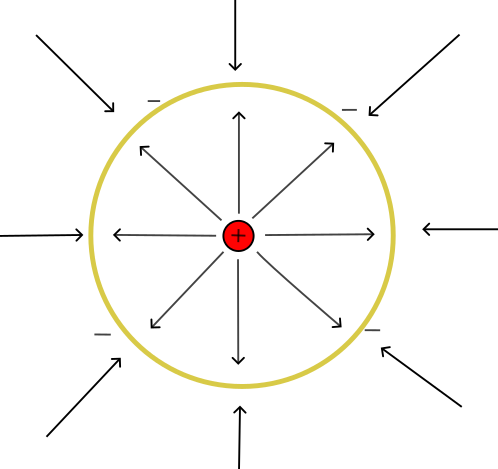
\includegraphics[scale=0.5]{a1}
	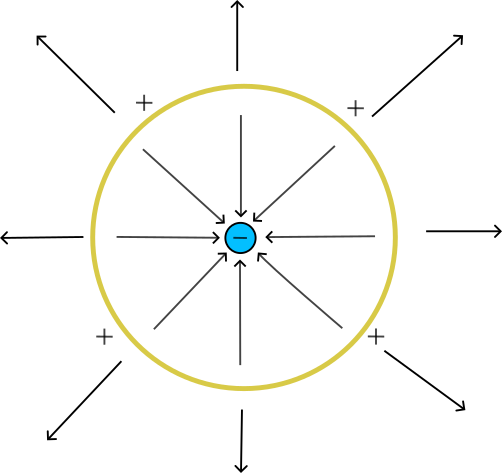
\includegraphics[scale=0.5]{a2}
	\caption{Líneas del campo eléctrico formado en la Figura \ref{fig:AyLE1} (izquierda) y la Figura \ref{fig:AyLE2} (derecha).}
\end{figure}

\newpage
\subsection{Dos cargas puntuales de diferente signo.}

\begin{figure}[h!]
	\centering
	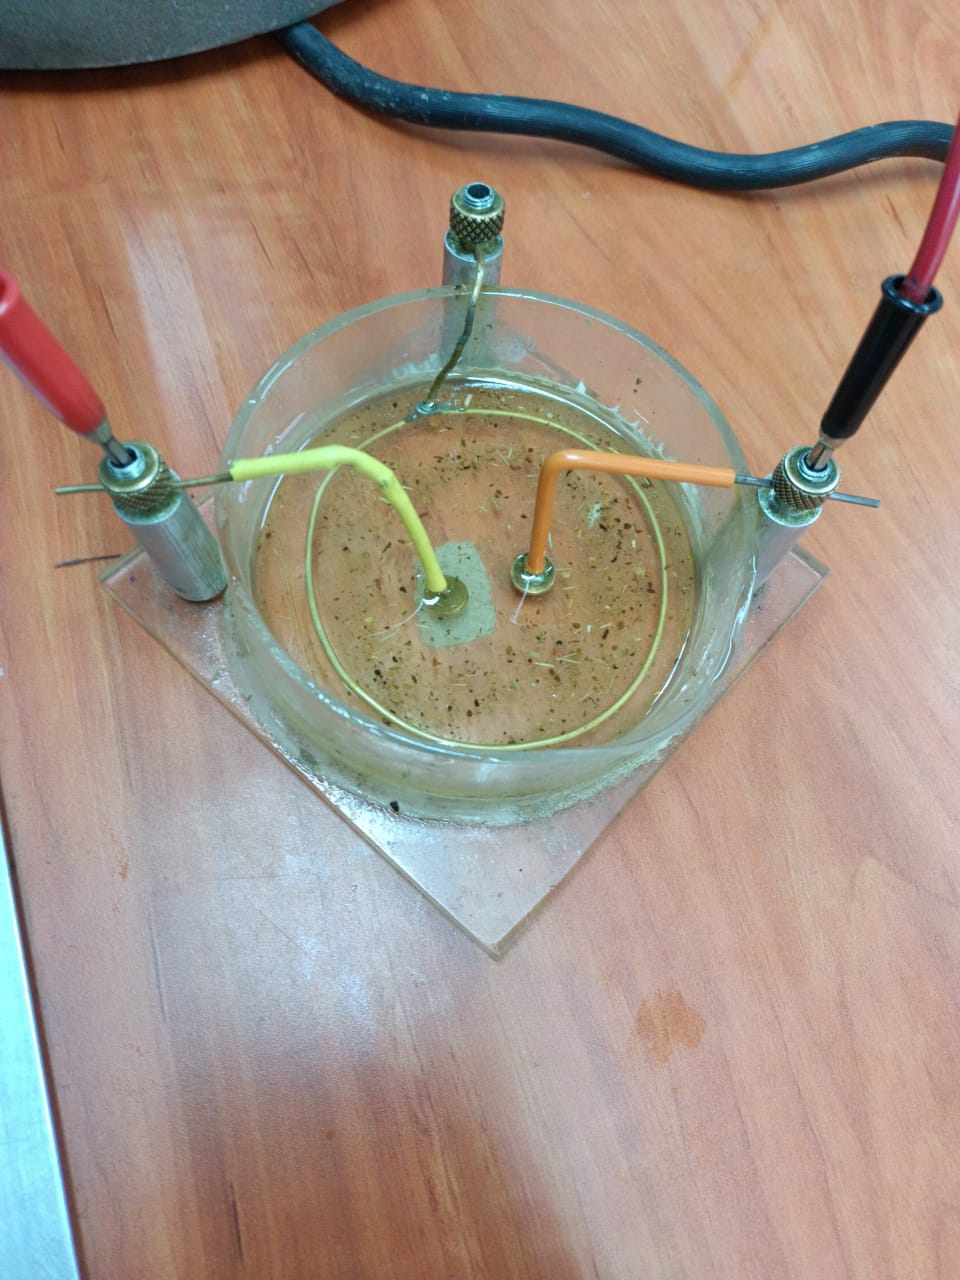
\includegraphics[scale=0.2]{Dos cargas Dif 1}
	\caption{Sistema con el generador apagado.}
\end{figure}

\begin{figure}[h!]
	\centering
	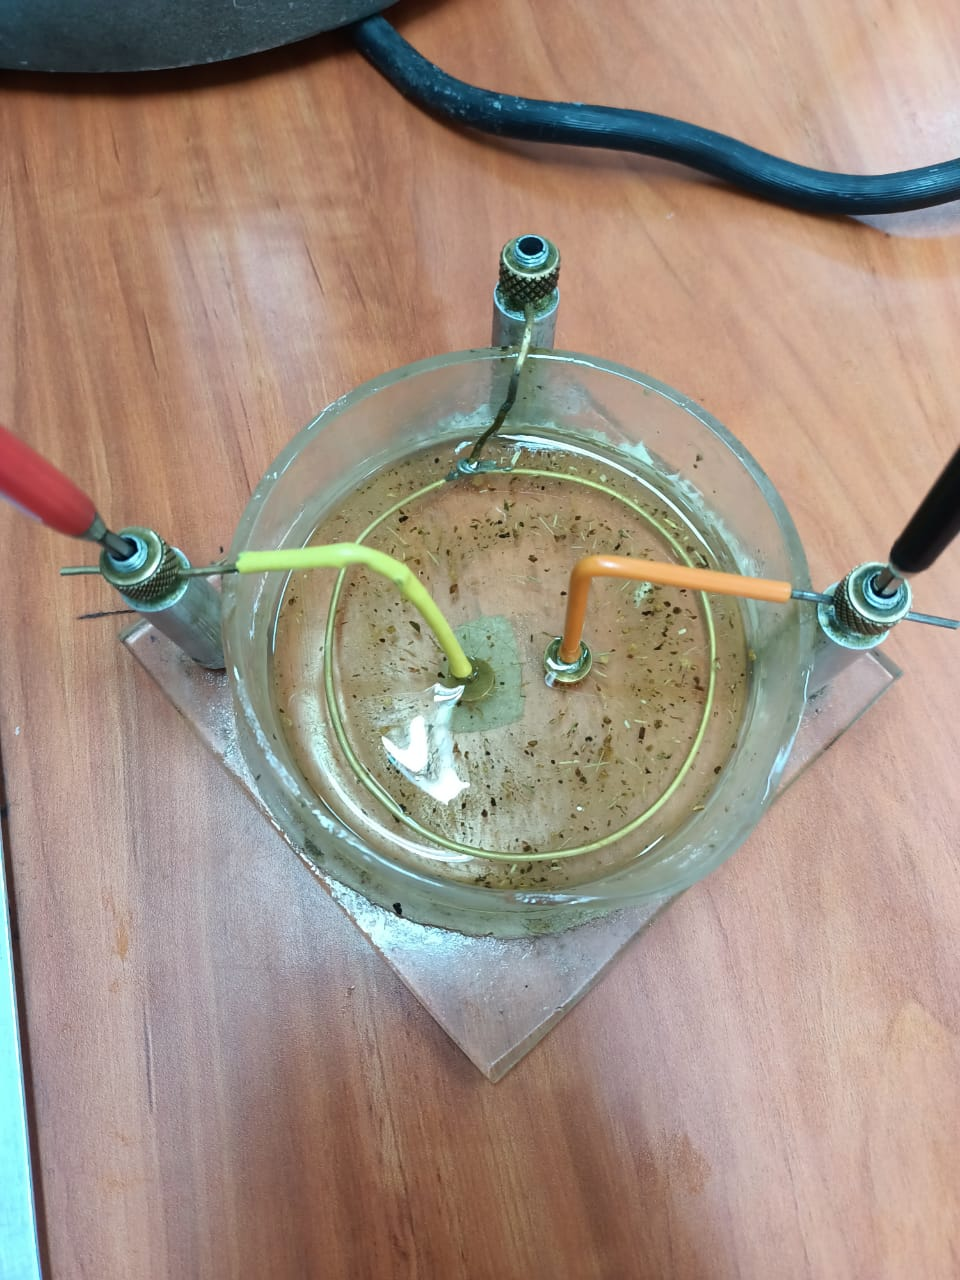
\includegraphics[scale=0.2]{Dos cargas Dif 2}
	\caption{Sistema con el generador encendido.}
	\label{fig:CDif1}
\end{figure}

En la Figura \ref{fig:CDif1} podemos observar ahora como el aserrín comienza a formar curvas. Nuevamente para describir mejor el comportamiento del campo eléctrico lo dibujaremos considerando la polaridad de los electrodos.

\begin{figure}[h!]
	\centering
	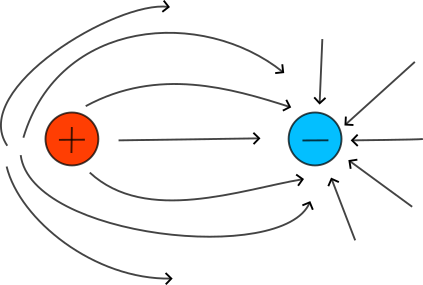
\includegraphics[scale=0.5]{b}
	\caption{Campo eléctrico formado en la Figura \ref{fig:CDif1}.}
	
\end{figure}

\newpage
\subsection{Dos cargas puntuales del mismo signo.}

\begin{figure}[h!]
	\centering
	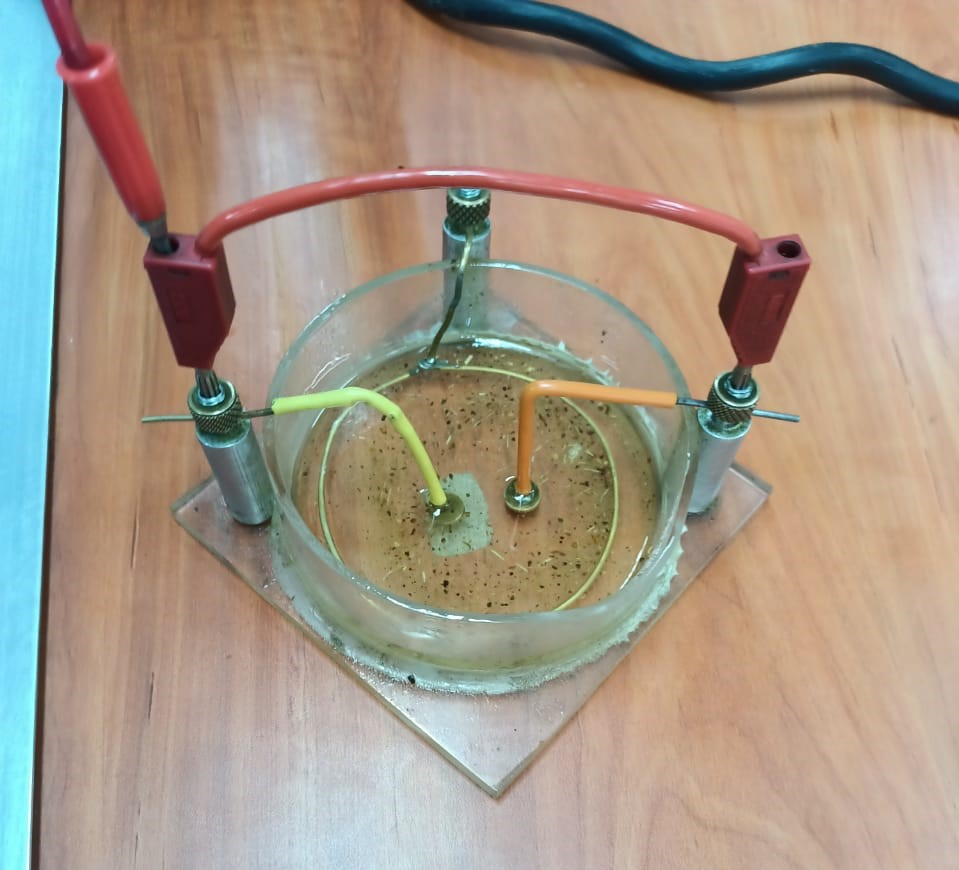
\includegraphics[scale=0.3]{Dos cargas Ig 1}
	\caption{Sistema con el generador apagado.}
	\label{fig:2CarIA}
\end{figure}

\begin{figure}[h!]
	\centering
	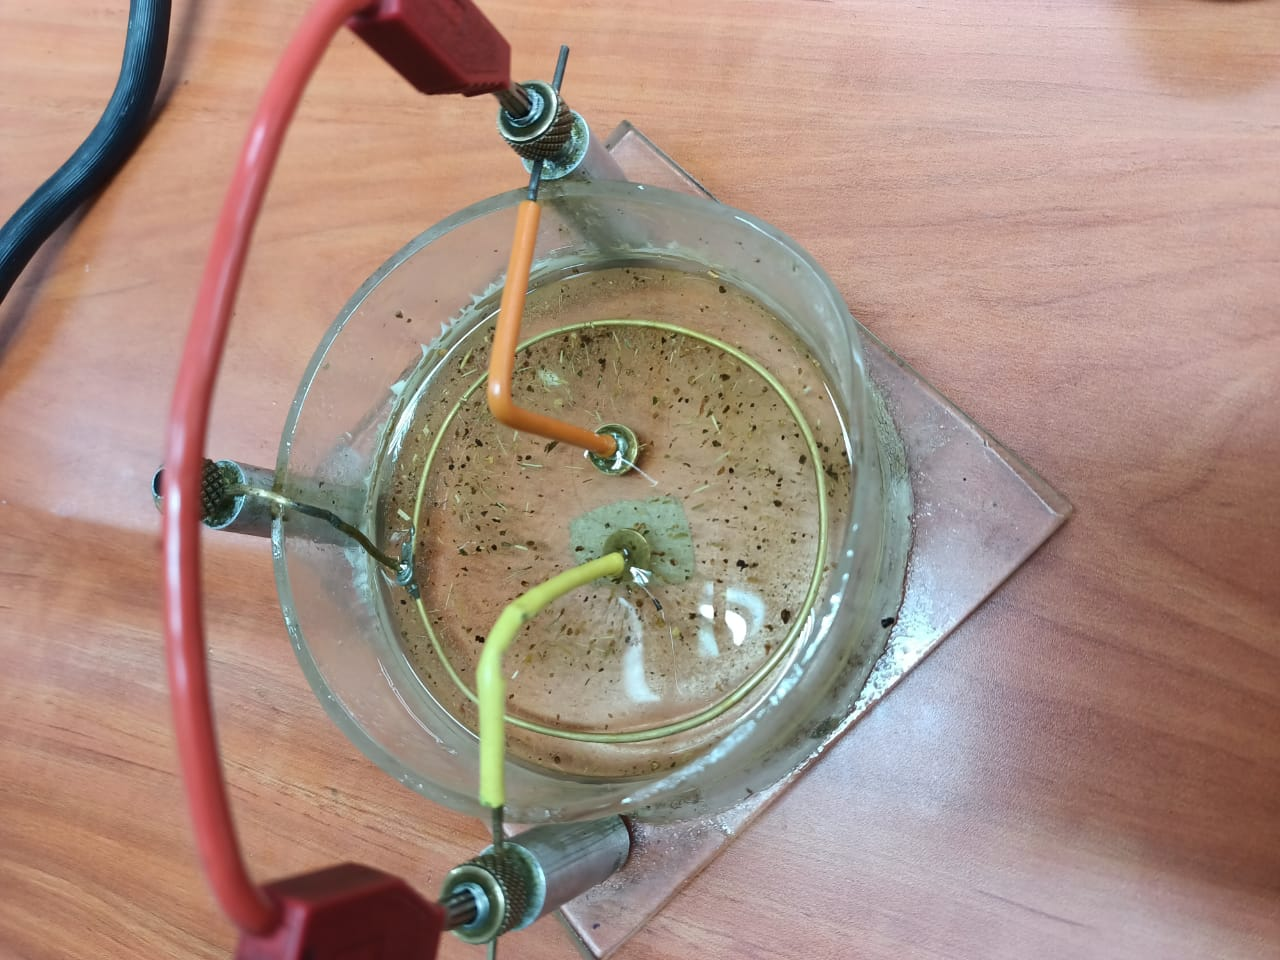
\includegraphics[scale=0.3]{Dos cargas Ig 2}
	\caption{Sistema con el generador encendido.}
	\label{fig:2CarI}
\end{figure}

En la Figura \ref{fig:2CarIA} podemos determinar que las dos cargas son positivas y en la Figura \ref{fig:2CarI} observamos nuevamente la formación de líneas pero con la particularidad que la parte media entre las dos cargas está vacía esto por la acción de la repulsión.

\begin{figure}
	\centering
	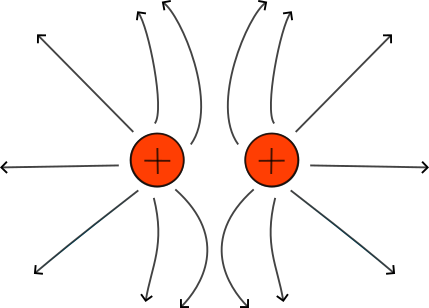
\includegraphics[scale=0.5]{c}
	\caption{Campo eléctrico formado en la Figura \ref{fig:2CarI}.}
\end{figure}

\subsection{Dos placas paralelas cargadas de diferente signo.}

\begin{figure}[h!]
	\centering
	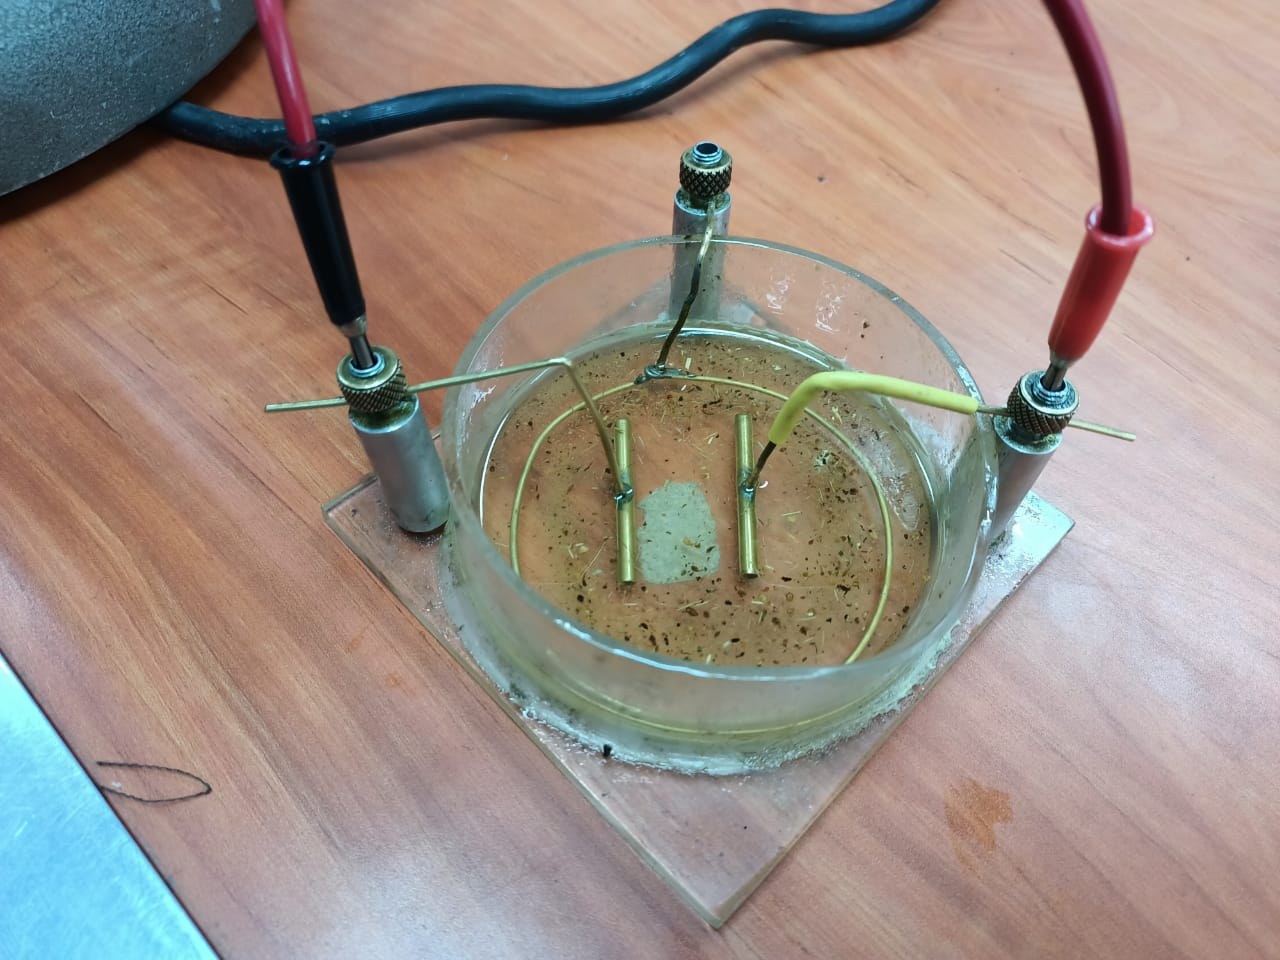
\includegraphics[scale=0.2]{Dos placas 1}
	\caption{Sistema con el generador apagado.}
\end{figure}

\begin{figure}[h!]
	\centering
	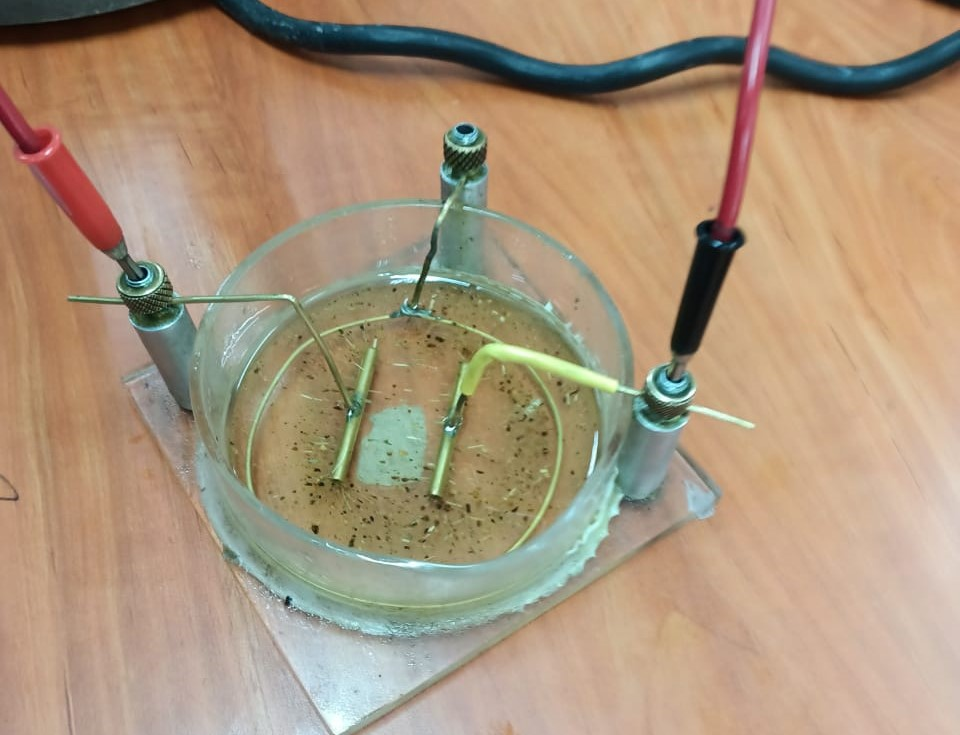
\includegraphics[scale=0.3]{Dos placas 2}
	\caption{Sistema con el generador encendido.}
	\label{fig:DosPlacas}
\end{figure}

En la figura \ref{fig:DosPlacas} podemos observar como entre las placas el aserrín forma la líneas paralelas y al rededor de los electrodos forman curvas.

\begin{figure}[h!]
	\centering
	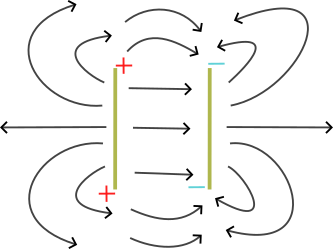
\includegraphics[scale=0.5]{d}
	\caption{Campo eléctrico formado en la Figura \ref{fig:DosPlacas}.}
\end{figure}

\newpage
\subsection{Dos arillos circulares cargados con diferente carga}

\begin{figure}[h!]
	\centering
	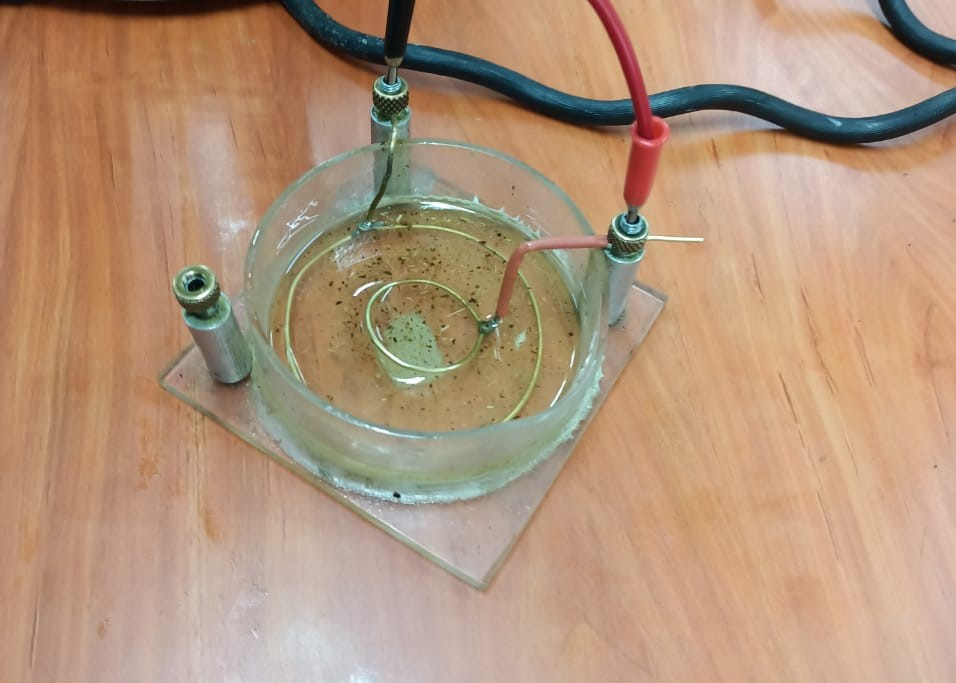
\includegraphics[scale=0.4]{Dos arillos 1}
	\caption{Sistema con el generador apagado.}
\end{figure}

\begin{figure}[h!]
	\centering
	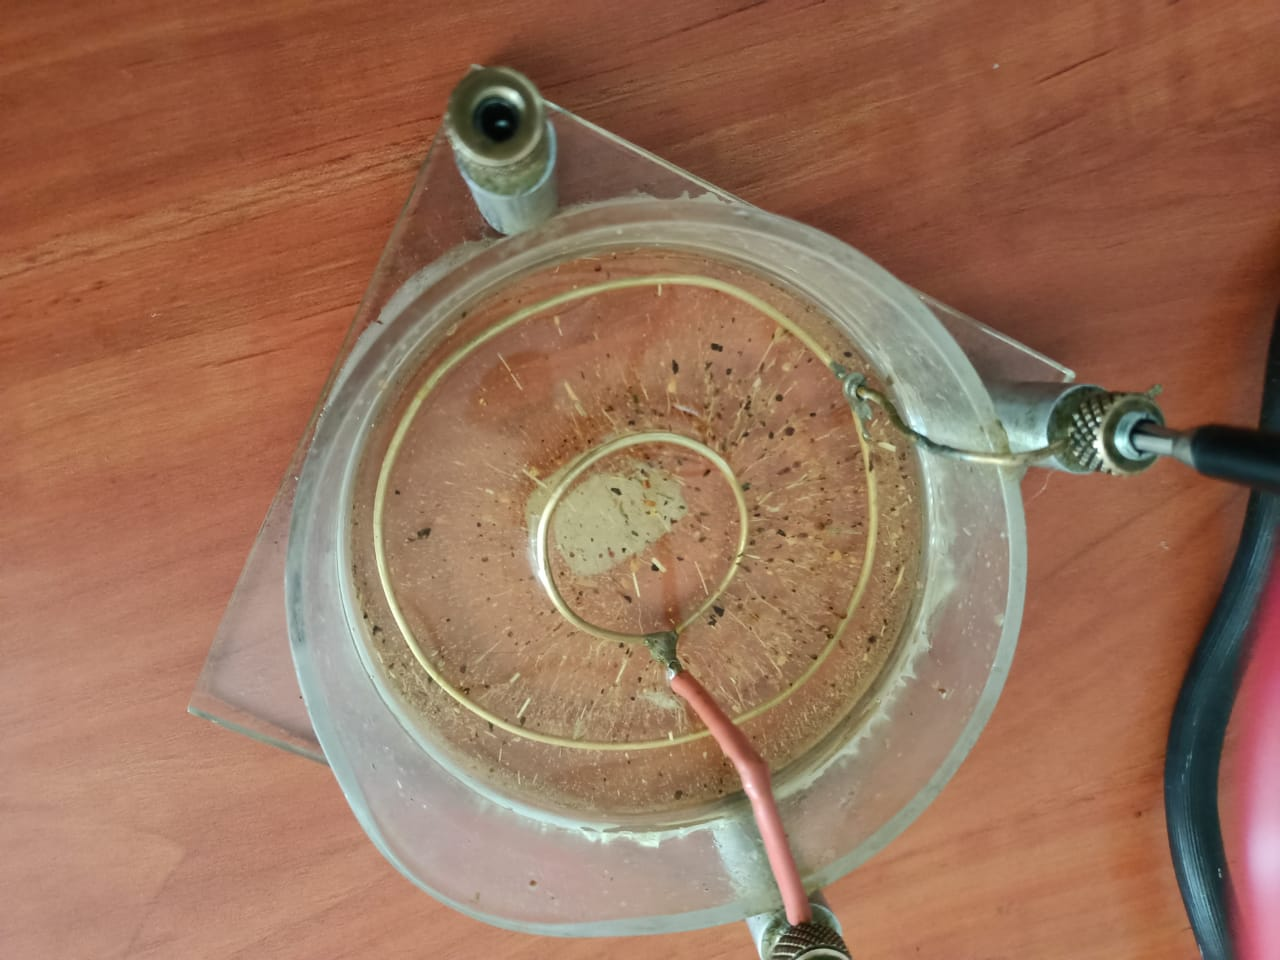
\includegraphics[scale=0.3]{Dos arillos 2}
	\caption{Sistema con el generador encendido.}
	\label{fig:DosArillos}
\end{figure}

En la figura \ref{fig:DosArillos} podemos observar que el aserrín forma líneas de tal manera que parece que dibujan el radio tanto del círculo más grande y el del más pequeño.

\begin{figure}[h!]
	\centering
	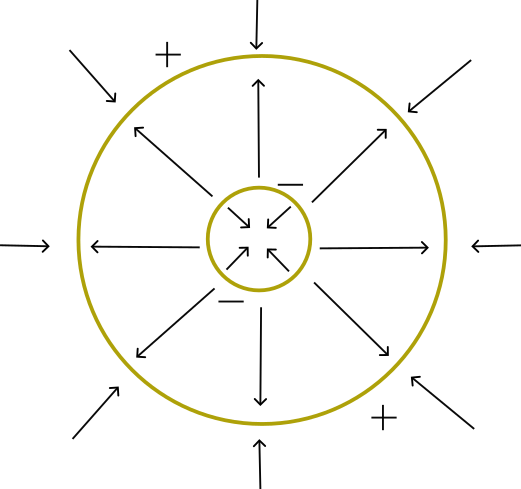
\includegraphics[scale=0.5]{e}
	\caption{Campo eléctrico formado en la figura \ref{fig:DosArillos}}
\end{figure}

\end{document}
